\begin{figure}[htbp]
\centering
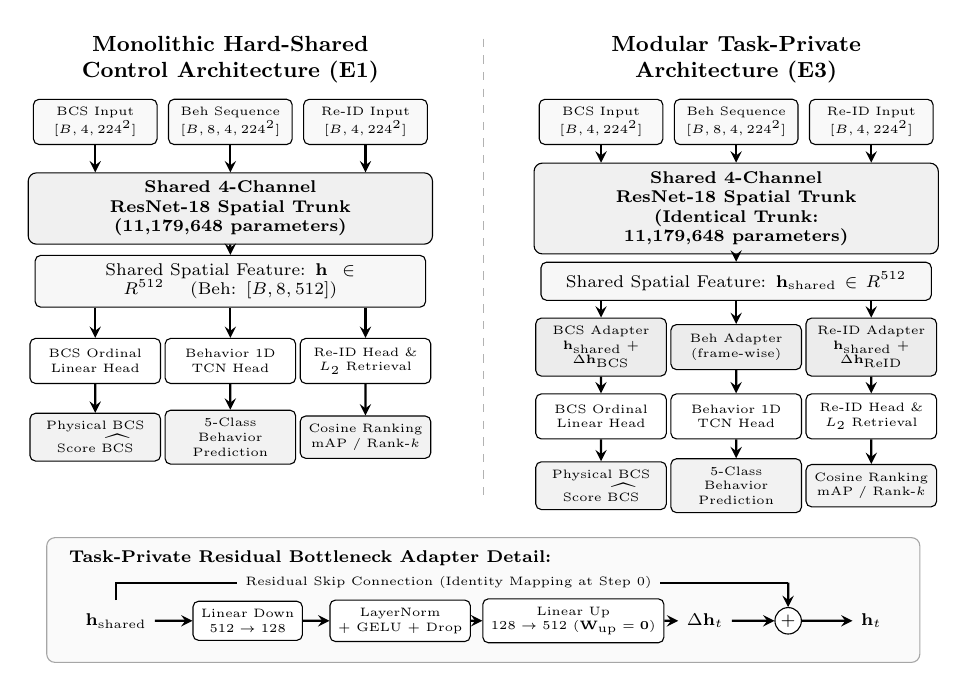
\begin{tikzpicture}[
  scale=0.88, every node/.style={transform shape},
  title/.style={font=\bfseries\small, align=center},
  inbox/.style={draw, rectangle, rounded corners=2pt, align=center, font=\tiny, text width=1.55cm, minimum height=0.55cm, fill=gray!5},
  trunk/.style={draw, rectangle, rounded corners=3pt, align=center, font=\scriptsize\bfseries, text width=5.6cm, minimum height=0.75cm, fill=gray!12},
  feat/.style={draw, rectangle, rounded corners=2pt, align=center, font=\scriptsize, text width=5.4cm, minimum height=0.55cm, fill=gray!6},
  head/.style={draw, rectangle, rounded corners=2pt, align=center, font=\tiny, text width=1.65cm, minimum height=0.65cm},
  outbox/.style={draw, rectangle, rounded corners=2pt, align=center, font=\tiny, text width=1.65cm, minimum height=0.55cm, fill=gray!10},
  adapter/.style={draw, rectangle, rounded corners=2pt, align=center, font=\tiny, text width=1.65cm, minimum height=0.65cm, fill=gray!15},
  arrow/.style={->, >=stealth, thick},
  line/.style={thick}
]

% ==================== LEFT: Hard-Shared MTL ====================
\node[title] at (2.85, 0.9) {Monolithic Hard-Shared\\Control Architecture (E1)};

\node[inbox] (e1_in1) at (0.9, 0) {BCS Input\\$[B,4,224^2]$};
\node[inbox] (e1_in2) at (2.85, 0) {Beh Sequence\\$[B,8,4,224^2]$};
\node[inbox] (e1_in3) at (4.8, 0) {Re-ID Input\\$[B,4,224^2]$};

\node[trunk] (e1_trunk) at (2.85, -1.25) {Shared 4-Channel ResNet-18 Spatial Trunk\\{\scriptsize (11,179,648 parameters)}};

\draw[arrow] (e1_in1.south) -- (e1_in1 |- e1_trunk.north);
\draw[arrow] (e1_in2.south) -- (e1_trunk.north);
\draw[arrow] (e1_in3.south) -- (e1_in3 |- e1_trunk.north);

\node[feat] (e1_feat) at (2.85, -2.3) {Shared Spatial Feature: $\mathbf{h} \in \mathbb{R}^{512}$ \quad (Beh: $[B, 8, 512]$)};
\draw[arrow] (e1_trunk) -- (e1_feat);

\node[head] (e1_h1) at (0.9, -3.45) {BCS Ordinal\\Linear Head};
\node[head] (e1_h2) at (2.85, -3.45) {Behavior 1D\\TCN Head};
\node[head] (e1_h3) at (4.8, -3.45) {Re-ID Head \&\\$L_2$ Retrieval};

\draw[arrow] (e1_feat.south -| e1_h1.north) -- (e1_h1.north);
\draw[arrow] (e1_feat.south) -- (e1_h2.north);
\draw[arrow] (e1_feat.south -| e1_h3.north) -- (e1_h3.north);

\node[outbox] (e1_o1) at (0.9, -4.55) {Physical BCS\\Score $\widehat{\mathrm{BCS}}$};
\node[outbox] (e1_o2) at (2.85, -4.55) {5-Class Behavior\\Prediction};
\node[outbox] (e1_o3) at (4.8, -4.55) {Cosine Ranking\\mAP / Rank-$k$};

\draw[arrow] (e1_h1) -- (e1_o1);
\draw[arrow] (e1_h2) -- (e1_o2);
\draw[arrow] (e1_h3) -- (e1_o3);

% ==================== RIGHT: Modular Task-Private MTL ====================
\node[title] at (10.15, 0.9) {Modular Task-Private\\Architecture (E3)};

\node[inbox] (e3_in1) at (8.2, 0) {BCS Input\\$[B,4,224^2]$};
\node[inbox] (e3_in2) at (10.15, 0) {Beh Sequence\\$[B,8,4,224^2]$};
\node[inbox] (e3_in3) at (12.1, 0) {Re-ID Input\\$[B,4,224^2]$};

\node[trunk] (e3_trunk) at (10.15, -1.25) {Shared 4-Channel ResNet-18 Spatial Trunk\\{\scriptsize (Identical Trunk: 11,179,648 parameters)}};

\draw[arrow] (e3_in1.south) -- (e3_in1 |- e3_trunk.north);
\draw[arrow] (e3_in2.south) -- (e3_trunk.north);
\draw[arrow] (e3_in3.south) -- (e3_in3 |- e3_trunk.north);

\node[feat] (e3_feat) at (10.15, -2.3) {Shared Spatial Feature: $\mathbf{h}_{\mathrm{shared}} \in \mathbb{R}^{512}$};
\draw[arrow] (e3_trunk) -- (e3_feat);

\node[adapter] (e3_ad1) at (8.2, -3.25) {BCS Adapter\\$\mathbf{h}_{\mathrm{shared}} + \Delta\mathbf{h}_{\mathrm{BCS}}$};
\node[adapter] (e3_ad2) at (10.15, -3.25) {Beh Adapter\\(frame-wise)};
\node[adapter] (e3_ad3) at (12.1, -3.25) {Re-ID Adapter\\$\mathbf{h}_{\mathrm{shared}} + \Delta\mathbf{h}_{\mathrm{ReID}}$};

\draw[arrow] (e3_feat.south -| e3_ad1.north) -- (e3_ad1.north);
\draw[arrow] (e3_feat.south) -- (e3_ad2.north);
\draw[arrow] (e3_feat.south -| e3_ad3.north) -- (e3_ad3.north);

\node[head] (e3_h1) at (8.2, -4.25) {BCS Ordinal\\Linear Head};
\node[head] (e3_h2) at (10.15, -4.25) {Behavior 1D\\TCN Head};
\node[head] (e3_h3) at (12.1, -4.25) {Re-ID Head \&\\$L_2$ Retrieval};

\draw[arrow] (e3_ad1) -- (e3_h1);
\draw[arrow] (e3_ad2) -- (e3_h2);
\draw[arrow] (e3_ad3) -- (e3_h3);

\node[outbox] (e3_o1) at (8.2, -5.25) {Physical BCS\\Score $\widehat{\mathrm{BCS}}$};
\node[outbox] (e3_o2) at (10.15, -5.25) {5-Class Behavior\\Prediction};
\node[outbox] (e3_o3) at (12.1, -5.25) {Cosine Ranking\\mAP / Rank-$k$};

\draw[arrow] (e3_h1) -- (e3_o1);
\draw[arrow] (e3_h2) -- (e3_o2);
\draw[arrow] (e3_h3) -- (e3_o3);

% ==================== DIVIDING LINE ====================
\draw[dashed, gray!60] (6.5, 1.2) -- (6.5, -5.5);

% ==================== BOTTOM INSET: Residual Adapter Detail ====================
\draw[rounded corners=3pt, fill=gray!4, draw=gray!70] (0.2, -6.0) rectangle (12.8, -7.8);
\node[font=\bfseries\scriptsize, anchor=west] at (0.4, -6.3) {Task-Private Residual Bottleneck Adapter Detail:};

\node[font=\scriptsize] (ad_in) at (1.2, -7.2) {$\mathbf{h}_{\mathrm{shared}}$};
\node[draw, rectangle, rounded corners=2pt, font=\tiny, align=center, fill=white] (ad_down) at (3.1, -7.2) {Linear Down\\$512 \to 128$};
\node[draw, rectangle, rounded corners=2pt, font=\tiny, align=center, fill=white] (ad_norm) at (5.3, -7.2) {LayerNorm\\+ GELU + Drop};
\node[draw, rectangle, rounded corners=2pt, font=\tiny, align=center, fill=white] (ad_up) at (7.8, -7.2) {Linear Up\\$128 \to 512$ ($\mathbf{W}_{\mathrm{up}}=\mathbf{0}$)};
\node[font=\scriptsize] (ad_dh) at (9.7, -7.2) {$\Delta\mathbf{h}_t$};
\node[draw, circle, inner sep=1pt, font=\scriptsize, fill=white] (ad_sum) at (10.9, -7.2) {$+$};
\node[font=\scriptsize] (ad_out) at (12.1, -7.2) {$\mathbf{h}_t$};

\draw[arrow] (ad_in) -- (ad_down);
\draw[arrow] (ad_down) -- (ad_norm);
\draw[arrow] (ad_norm) -- (ad_up);
\draw[arrow] (ad_up) -- (ad_dh);
\draw[arrow] (ad_dh) -- (ad_sum);
\draw[arrow] (ad_sum) -- (ad_out);

% Residual skip arrow
\draw[line] (1.2, -6.9) -- (1.2, -6.65) -- (10.9, -6.65);
\draw[arrow] (10.9, -6.65) -- (ad_sum.north);
\node[font=\tiny, fill=gray!4] at (6.0, -6.65) {Residual Skip Connection (Identity Mapping at Step 0)};

\end{tikzpicture}
\caption[Multi-task architecture comparison: hard-shared vs. modular]{Architectural comparison between the monolithic hard-shared multi-task control (E1, left) and the modular task-private multi-task architecture (E3, right). Both architectures share an identical four-channel ResNet-18 spatial trunk and task prediction heads. E3 inserts an independent residual bottleneck adapter (bottom detail) between the shared 512-dimensional representation and each task-specific head, initialized as an identity mapping ($\mathbf{W}_{\mathrm{up}}=\mathbf{0}$).}
\label{fig:mtl_architecture_comparison}
\end{figure}
